\begin{center}

\includegraphics[width=0.6\textwidth]{content/3/chapter6/images/7.png}\\
Cippi studies the atomics
\end{center}

Atomics receives a few important extensions in C++20. Probably the most important ones are atomic references and atomic smart pointers.

\subsubsubsection{6.2.1\hspace{0.2cm} std::atomic\_ref}

The class template std::atomic\_ref applies atomic operations to the referenced object.

Concurrent writing and reading of an atomic object ensures that there is no data race. The lifetime of the referenced object must exceed the lifetime of the atomic\_ref. When any atomic\_ref is accessing an object, all other accesses to the object must use an atomic\_ref. In addition, no subobject of the atomic\_ref-accessed object may be accessed by another atomic\_ref.

\hspace*{\fill} \\ %插入空行
\noindent
\textbf{6.2.1.1\hspace{0.2cm} Motivation}

Stop. You may think that using a reference inside an atomic would do the job. Unfortunately not.

In the following program, I have a class ExpensiveToCopy, which includes a counter. The counter is concurrently incremented by a few threads. Consequently, counter has to be protected.

\hspace*{\fill} \\ %插入空行
\noindent
Using an atomic reference
\begin{lstlisting}[style=styleCXX]
// atomicReference.cpp

#include <atomic>
#include <iostream>
#include <random>
#include <thread>
#include <vector>

struct ExpensiveToCopy {
	int counter{};
};

int getRandom(int begin, int end) {
	
	std::random_device seed; // initial seed
	std::mt19937 engine(seed()); // generator
	std::uniform_int_distribution<> uniformDist(begin, end);
	
	return uniformDist(engine);
}

void count(ExpensiveToCopy& exp) {

	std::vector<std::thread> v;
	std::atomic<int> counter{exp.counter};
	
	for (int n = 0; n < 10; ++n) {
		v.emplace_back([&counter] {
			auto randomNumber = getRandom(100, 200);
			for (int i = 0; i < randomNumber; ++i) { ++counter; }
		});
	}
	
	for (auto& t : v) t.join();

}

int main() {
	
	std::cout << '\n';
	
	ExpensiveToCopy exp;
	count(exp);
	std::cout << "exp.counter: " << exp.counter << '\n';
	
	std::cout << '\n';

}
\end{lstlisting}

Variable exp (line 42) is the expensive-to-copy object. For performance reasons, the function count (line 22) takes exp by reference. Function count initializes the std::atomic<int> with exp.counter (line 25). The following lines create 10 threads (line 27), each performing the lambda expression, which takes counter by reference. The lambda expression gets a random number between 100 and 200 (line 29) and increments the counter exactly as often. The function getRandom (line 13) starts with an initial seed and creates via the random-number generator \href{https://en.wikipedia.org/wiki/Mersenne_Twister}{Mersenne Twister} a uniform distributed number between 100 and 200.

In the end, the exp.counter (line 44) should have an approximate value of 1500 because ten threads increment on average 150 times. Executing the program on the \href{https://wandbox.org/}{Wandbox online compiler} gives me a surprising result.

\begin{center}
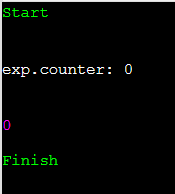
\includegraphics[width=0.4\textwidth]{content/3/chapter6/images/8.png}\\
Surprise with an atomic reference
\end{center}

The counter is 0. What is happening? The issue is in line 25. The initialization in the expression std::atomic<int> counter{exp.counter} creates a copy. The following small program exemplifies the issue.

\hspace*{\fill} \\ %插入空行
\noindent
Copying the reference
\begin{lstlisting}[style=styleCXX]
// atomicRefCopy.cpp

#include <atomic>
#include <iostream>

int main() {

	std::cout << '\n';
	
	int val{5};
	int& ref = val;
	std::atomic<int> atomicRef(ref);
	++atomicRef;
	std::cout << "ref: " << ref << '\n';
	std::cout << "atomicRef.load(): " << atomicRef.load() << '\n';
	
	std::cout << '\n';

}
\end{lstlisting}

The increment operation in line 13 does not address the reference ref (line 11). The value of ref is not changed.

\begin{center}
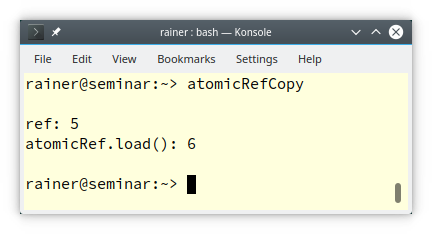
\includegraphics[width=0.4\textwidth]{content/3/chapter6/images/9.png}\\
Copying the reference
\end{center}

Replacing the std::atomic<int> with std::atomic\_ref<int> solves the issue.

\hspace*{\fill} \\ %插入空行
\noindent
Using a std::atomic\_ref
\begin{lstlisting}[style=styleCXX]
// atomicRef.cpp

#include <atomic>
#include <iostream>
#include <random>
#include <thread>
#include <vector>

struct ExpensiveToCopy {
	int counter{};
};

int getRandom(int begin, int end) {
	std::random_device seed; // initial randomness
	std::mt19937 engine(seed()); // generator
	std::uniform_int_distribution<> uniformDist(begin, end);
	
	return uniformDist(engine);
}

void count(ExpensiveToCopy& exp) {
	
	std::vector<std::thread> v;
	std::atomic_ref<int> counter{exp.counter};
	
	for (int n = 0; n < 10; ++n) {
		v.emplace_back([&counter] {
			auto randomNumber = getRandom(100, 200);
			for (int i = 0; i < randomNumber; ++i) { ++counter; }
		});
	}

	for (auto& t : v) t.join();
}

int main() {
	
	std::cout << '\n';
	
	ExpensiveToCopy exp;
	count(exp);
	std::cout << "exp.counter: " << exp.counter << '\n';
	
	std::cout << '\n';
}
\end{lstlisting}

Now, the value of counter is as expected:

\begin{center}
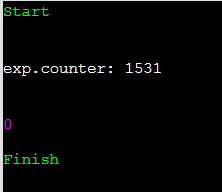
\includegraphics[width=0.4\textwidth]{content/3/chapter6/images/10.png}\\
The expected result with std::atomic\_ref
\end{center}

In keeping with \href{https://en.cppreference.com/w/cpp/atomic/atomic}{std::atomic}, type std::atomic\_ref can be specialized and supports specializations for the built-in data types.

\hspace*{\fill} \\ %插入空行
\noindent
\textbf{6.2.1.2\hspace{0.2cm} Specializations of std::atomic\_ref}

You can specialize std::atomic\_ref for user-defined types, use partial specializations for pointer types, or full specializations for arithmetic types such as integral or floating-point types.

\hspace*{\fill} \\ %插入空行
\noindent
\textbf{6.2.1.2.1\hspace{0.2cm} Primary Template}

The primary template std::atomic\_ref can be instantiated with a \href{https://en.cppreference.com/w/cpp/types/is_trivially_copyable}{TriviallyCopyable} type T.

\begin{lstlisting}[style=styleCXX]
struct Counters {
	int a;
	int b;
};

Counter counter;
std::atomic_ref<Counters> cnt(counter);
\end{lstlisting}

\hspace*{\fill} \\ %插入空行
\noindent
\textbf{6.2.1.2.2\hspace{0.2cm} Partial Specializations for Pointer Types}

The standard provides partial specializations for a pointer type: std::atomic\_ref<T*>.

\hspace*{\fill} \\ %插入空行
\noindent
\textbf{6.2.1.2.3\hspace{0.2cm} Specializations for Arithmetic Types}

The standard provides specialization for the integral and floating-point types: std::atomic\_ref<arithmetic type>.

\begin{itemize}
\item 
Character types: char, char8\_t (C++20), char16\_t, char32\_t, and wchar\_t

\item 
Standard signed-integer types: signed char, short, int, long, and long long

\item 
Standard unsigned-integer types: unsigned char, unsigned short, unsigned int, unsigned long, and unsigned long long

\item 
Additional integer types, defined in the header \href{http://en.cppreference.com/w/cpp/header/cstdint}{<cstdint>}:
\begin{itemize}
\item 
int8\_t, int16\_t, int32\_t, and int64\_t (signed integer with exactly 8, 16, 32, and 64 bits)

\item 
uint8\_t, uint16\_t, uint32\_t, and uint64\_t (unsigned integer with exactly 8, 16, 32, and 64 bits)

\item 
int\_fast8\_t, int\_fast16\_t, int\_fast32\_t, and int\_fast64\_t (fastest signed integer with at least 8, 16, 32, and 64 bits)

\item 
uint\_fast8\_t, uint\_fast16\_t, uint\_fast32\_t, and uint\_fast64\_t (fastest unsigned integer with at least 8, 16, 32, and 64 bits)

\item 
int\_least8\_t, int\_least16\_t, int\_least32\_t, and int\_least64\_t (smallest signed integer with at least 8, 16, 32, and 64 bits)

\item 
uint\_least8\_t, uint\_least16\_t, uint\_least32\_t, and uint\_least64\_t (smallest unsigned integer with at least 8, 16, 32, and 64 bits)

\item 
intmax\_t, and uintmax\_t (maximum signed and unsigned integer)

\item 
intptr\_t, and uintptr\_t (signed and unsigned integer for holding a pointer)
\end{itemize}

\item 
Standard floating-point types: float, double, and long double
\end{itemize}

\hspace*{\fill} \\ %插入空行
\noindent
\textbf{6.2.1.2.4\hspace{0.2cm} All Atomic Operations}

First, here is the list of all operations on atomic\_ref.



\subsubsubsection{6.2.2\hspace{0.2cm} Atomic Smart Pointer}

\subsubsubsection{6.2.3\hspace{0.2cm} std::atomic\_flag Extensions}

\subsubsubsection{6.2.4\hspace{0.2cm} std::atomic Extensions}























